% Defense deck, CIS 6270 Project 1.
%
% The assignment fixes the structure: slides run in order from 1a to 3e, each carrying its
% label in the TOP-RIGHT corner, with numbered on-slide citations listed in a very small font
% at the BOTTOM-RIGHT, and a bibliography slide at the end. Items with two slides use
% "1c (i)" / "1c (ii)".
%
% Every table and number here \input{}s the SAME generated fragments as the paper, so a slide
% cannot disagree with it: regenerate with `python3 scripts/make_tables.py` and recompile.
%
% Build: cd slides && pdflatex defense && pdflatex defense
%
% Speaking split: slides/README.md (four speakers x four slides, about 13.5 min against the
% hard 15-minute limit). \note{} blocks are preparation only, not used at the defense.

\documentclass[aspectratio=169,10pt]{beamer}
\usetheme{default}
\usecolortheme{seahorse}
\setbeamertemplate{navigation symbols}{}
\setbeamertemplate{footline}{}
\setbeamerfont{frametitle}{size=\large}
\setbeamerfont{normal text}{size=\small}
\usefonttheme{professionalfonts}
\setbeamercolor{frametitle}{bg=}
\usepackage{booktabs}
\usepackage{amsmath}
\usepackage{graphicx}
\usepackage[T1]{fontenc}
\usepackage{tikz}
\usetikzlibrary{positioning,arrows.meta,fit,calc}

% ---- the label (top right) and the source list (bottom right) -------------------
% \lab{1a} puts the required item label in the top-right corner of the current frame.
\newcommand{\lab}[1]{%
  \begin{textblock*}{1.3cm}(14.5cm,0.28cm)
    \raggedleft\bfseries\small\textcolor{gray}{#1}
  \end{textblock*}}
% \srcs{...} puts the numbered source list in the bottom-right, in a very small font.
% Numbering restarts per slide, which the assignment explicitly permits.
\newcommand{\srcs}[1]{%
  \begin{textblock*}{11cm}(4.6cm,8.62cm)
    \raggedleft\fontsize{4.8}{5.6}\selectfont\textcolor{gray}{#1}
  \end{textblock*}}
\usepackage[absolute,overlay]{textpos}

% The table fragments are shared verbatim with the paper, so they contain paper-style
% \citep{...} keys. The deck has no bibliography backend and carries its own numbered
% on-slide citations in \srcs{} instead, as the assignment requires, so the keys are
% suppressed here rather than dropped from the shared source.
\providecommand{\citep}[1]{}
\providecommand{\citet}[1]{}
\setlength{\TPHorizModule}{1cm}\setlength{\TPVertModule}{1cm}

\title{\textbf{VANISH: Vanishing-Factor Ablation of Non-tangent Flows in Simplex and Hypercube}}
\subtitle{\normalsize Learned flows leave bounded domains; a vanishing factor restores feasibility, not quality}
\author{Roshan Bellary \and Audhav Durai \and Chang-Uk Jeong \and Pedram Bayat}
\institute{\small CIS 6270, University of Pennsylvania}
\date{30 September 2026}

% Generated by scripts/make_tables.py. Do not edit.
\newcommand{\BaseKmerCodon}{0.127}
\newcommand{\BaseKmerDna}{0.894}
\newcommand{\BaseKmerProt}{0.753}
\newcommand{\BaseKmerTwoCodon}{0.13}
\newcommand{\BaseKmerTwoDna}{0.89}
\newcommand{\BaseKmerTwoProt}{0.75}
\newcommand{\BaseViolCodon}{1.000}
\newcommand{\BaseViolDna}{0.713}
\newcommand{\BaseViolDnaFifty}{0.68}
\newcommand{\BaseViolDnaTen}{0.24}
\newcommand{\BaseViolPctDna}{71}
\newcommand{\BaseViolProt}{0.967}
\newcommand{\BaseViolTwoCodon}{1.00}
\newcommand{\BaseViolTwoDna}{0.71}
\newcommand{\BaseViolTwoProt}{0.97}
\newcommand{\BaseXMin}{0.979}
\newcommand{\BaselinesFixed}{1}
\newcommand{\BestKmerCodon}{Dirichlet FM}
\newcommand{\BestKmerDna}{Fisher-Flow}
\newcommand{\BestKmerProt}{Dirichlet FM}
\newcommand{\BigBaseCodon}{0.182}
\newcommand{\BigBaseProt}{0.885}
\newcommand{\BigHardGainCodon}{-0.027}
\newcommand{\BigHardGainProt}{+0.017}
\newcommand{\BigSeeds}{3}
\newcommand{\CommitCodon}{0.048}
\newcommand{\CommitDna}{0.055}
\newcommand{\CommitProt}{0.056}
\newcommand{\CommitSettledHi}{96}
\newcommand{\CommitSettledLo}{88}
\newcommand{\CommitStep}{5}
\newcommand{\CommitWasted}{95}
\newcommand{\DiffHam}{0.69 / 0.90 / 0.94}
\newcommand{\DiffHamTen}{0.46 / 0.60 / 0.79}
\newcommand{\DirichletCNonfinite}{0}
\newcommand{\DirichletKL}{0.005 / 0.015 / 0.045}
\newcommand{\DirichletKLCodon}{0.04}
\newcommand{\DirichletKmer}{0.901 / 0.906 / 0.447}
\newcommand{\DirichletKmerCodon}{0.447}
\newcommand{\DirichletKmerOld}{0.714 / 0.271 / 0.448}
\newcommand{\DirichletKmerState}{0.904 / 0.911 / 0.375}
\newcommand{\DirichletViol}{0.000 / 0.000 / 0.000}
\newcommand{\DirichletViolOld}{0.006 / 0.843 / 1.000}
\newcommand{\DirichletVsBaseCodon}{$+0.320\,[+0.300, +0.340]$}
\newcommand{\DirichletVsBaseDna}{$+0.007\,[-0.081, +0.102]$}
\newcommand{\DirichletVsBaseProt}{$+0.154\,[+0.113, +0.201]$}
\newcommand{\DirichletVsOursCodon}{$+0.250\,[+0.230, +0.269]$}
\newcommand{\DirichletVsOursDna}{$+0.003\,[-0.072, +0.075]$}
\newcommand{\DirichletVsOursPosCodon}{8}
\newcommand{\DirichletVsOursPosDna}{4}
\newcommand{\DirichletVsOursPosProt}{8}
\newcommand{\DirichletVsOursProt}{$+0.041\,[+0.020, +0.071]$}
\newcommand{\DropCenterCICodon}{$+0.009\,[-0.010, +0.031]$}
\newcommand{\DropCenterCodonN}{8}
\newcommand{\DropCenterCodonPos}{4}
\newcommand{\DropCenterCodonT}{$+0.009\,[-0.018, +0.036]$}
\newcommand{\EndpointCollapseCodon}{5}
\newcommand{\EndpointCollapseProt}{3}
\newcommand{\EndpointRwCollapseCodon}{6}
\newcommand{\EndpointRwCollapseProt}{3}
\newcommand{\FMHam}{0.75 / 0.94 / 0.98}
\newcommand{\FMHamTen}{0.75 / 0.91 / 0.87}
\newcommand{\FisherCodonNew}{0.295}
\newcommand{\FisherCodonOld}{0.421}
\newcommand{\FisherFixed}{1}
\newcommand{\FisherKL}{0.005 / 0.015 / 0.042}
\newcommand{\FisherKmer}{0.909 / 0.886 / 0.295}
\newcommand{\FisherKmerOld}{0.967 / 0.908 / 0.421}
\newcommand{\FisherViol}{0.000 / 0.000 / 0.000}
\newcommand{\FisherViolEuclid}{0.238 / 0.727 / 0.887}
\newcommand{\FisherViolHi}{100}
\newcommand{\FisherViolLo}{79.5}
\newcommand{\FisherViolOld}{0.795 / 0.985 / 1.000}
\newcommand{\FisherVsBaseCodon}{$+0.168\,[+0.145, +0.193]$}
\newcommand{\FisherVsBaseDna}{$+0.015\,[-0.035, +0.068]$}
\newcommand{\FisherVsBaseProt}{$+0.133\,[+0.089, +0.179]$}
\newcommand{\FisherVsOursCodon}{$+0.098\,[+0.080, +0.114]$}
\newcommand{\FisherVsOursDna}{$+0.011\,[-0.030, +0.045]$}
\newcommand{\FisherVsOursPosCodon}{8}
\newcommand{\FisherVsOursPosDna}{5}
\newcommand{\FisherVsOursPosProt}{5}
\newcommand{\FisherVsOursProt}{$+0.020\,[+0.001, +0.042]$}
\newcommand{\GRBestGammaDna}{0.1}
\newcommand{\GRBestGammaProt}{0.03}
\newcommand{\GRHamCIDna}{$-0.215\,[-0.221, -0.211]$}
\newcommand{\GRHamCIProt}{$-0.102\,[-0.110, -0.096]$}
\newcommand{\GRHamDefDna}{0.53}
\newcommand{\GRHamDefProt}{0.84}
\newcommand{\GRHamHighDna}{0.44}
\newcommand{\GRHamHighProt}{0.72}
\newcommand{\GRHamLowDna}{0.74}
\newcommand{\GRHamLowProt}{0.94}
\newcommand{\GRHamMidDna}{0.69}
\newcommand{\GRHamMidProt}{0.92}
\newcommand{\GRHamZeroDna}{0.75}
\newcommand{\GRHamZeroProt}{0.94}
\newcommand{\GRHitCIDna}{$+0.908\,[+0.870, +0.933]$}
\newcommand{\GRHitCIProt}{$+0.974\,[+0.965, +0.981]$}
\newcommand{\GRHitDefDna}{1.00}
\newcommand{\GRHitDefProt}{1.00}
\newcommand{\GRHitHighDna}{1.00}
\newcommand{\GRHitHighProt}{1.00}
\newcommand{\GRHitLowDna}{0.30}
\newcommand{\GRHitLowProt}{0.55}
\newcommand{\GRHitMidDna}{0.93}
\newcommand{\GRHitMidProt}{1.00}
\newcommand{\GRHitZeroDna}{0.09}
\newcommand{\GRHitZeroProt}{0.03}
\newcommand{\GRKmerCIDna}{$-0.860\,[-0.900, -0.819]$}
\newcommand{\GRKmerCIProt}{$-0.638\,[-0.661, -0.615]$}
\newcommand{\GRKmerDefDna}{0.04}
\newcommand{\GRKmerDefProt}{0.22}
\newcommand{\GRKmerHiCIDna}{$+0.060\,[-0.058, +0.169]$}
\newcommand{\GRKmerHiCIProt}{$-0.067\,[-0.100, -0.031]$}
\newcommand{\GRKmerHiDefDna}{0.65}
\newcommand{\GRKmerHiDefProt}{0.53}
\newcommand{\GRKmerHiHighDna}{0.55}
\newcommand{\GRKmerHiHighProt}{0.50}
\newcommand{\GRKmerHiLowDna}{0.92}
\newcommand{\GRKmerHiLowProt}{0.74}
\newcommand{\GRKmerHiMidDna}{0.94}
\newcommand{\GRKmerHiMidProt}{0.68}
\newcommand{\GRKmerHiZeroDna}{0.59}
\newcommand{\GRKmerHiZeroProt}{0.60}
\newcommand{\GRKmerHighDna}{0.04}
\newcommand{\GRKmerHighProt}{0.27}
\newcommand{\GRKmerLowDna}{0.71}
\newcommand{\GRKmerLowProt}{0.70}
\newcommand{\GRKmerMidDna}{0.37}
\newcommand{\GRKmerMidProt}{0.38}
\newcommand{\GRKmerZeroDna}{0.90}
\newcommand{\GRKmerZeroProt}{0.86}
\newcommand{\GRSecDna}{69}
\newcommand{\GRSecProt}{71}
\newcommand{\GRSeeds}{8}
\newcommand{\GRTargetDefDna}{0.96}
\newcommand{\GRTargetDefProt}{0.95}
\newcommand{\GRTargetHighDna}{1.00}
\newcommand{\GRTargetHighProt}{1.00}
\newcommand{\GRTargetLowDna}{0.59}
\newcommand{\GRTargetLowProt}{0.46}
\newcommand{\GRTargetMidDna}{0.74}
\newcommand{\GRTargetMidProt}{0.64}
\newcommand{\GRTargetZeroDna}{0.51}
\newcommand{\GRTargetZeroProt}{0.36}
\newcommand{\GRViolMaxDna}{0.000}
\newcommand{\GRViolMaxProt}{0.000}
\newcommand{\GammaKSp}{0.589/0.441/0.629}
\newcommand{\GammaShapes}{1.0/2.5/9.0}
\newcommand{\GuidHitMax}{1.000}
\newcommand{\GuidHitZero}{0.0136}
\newcommand{\GuidK}{8}
\newcommand{\GuidKLHi}{0.066}
\newcommand{\GuidKLLo}{0.046}
\newcommand{\GuidMassEuc}{5.99\times10^{-3}}
\newcommand{\GuidMassRatio}{21}
\newcommand{\GuidMassTan}{1.26\times10^{-1}}
\newcommand{\GuidN}{100{,}000}
\newcommand{\GuidNfe}{100}
\newcommand{\GuidPrior}{0.0018}
\newcommand{\GuidRareEuc}{12}
\newcommand{\GuidRareIdeal}{23}
\newcommand{\GuidRareNat}{40}
\newcommand{\GuidRareTan}{12}
\newcommand{\GuidStrengthRatio}{4}
\newcommand{\GuidViolEuc}{0.97}
\newcommand{\GuidViolNat}{0.77}
\newcommand{\GuidViolNatEightThree}{0.766}
\newcommand{\GuidViolTanEight}{1.000}
\newcommand{\GuidViolZero}{0.21}
\newcommand{\GumbelHamCodon}{0.947}
\newcommand{\GumbelHamProt}{0.878}
\newcommand{\GumbelKL}{0.010 / 0.606 / 0.982}
\newcommand{\GumbelKmer}{0.894 / 0.705 / 0.400}
\newcommand{\GumbelKmerOld}{0.586 / 0.499 / 0.041}
\newcommand{\GumbelKmerState}{0.903 / 0.876 / 0.224}
\newcommand{\GumbelStateHamProt}{0.940}
\newcommand{\GumbelViol}{0.000 / 0.000 / 0.000}
\newcommand{\GumbelViolOld}{0.488 / 0.907 / 1.000}
\newcommand{\GumbelVsBaseCodon}{$+0.273\,[+0.226, +0.320]$}
\newcommand{\GumbelVsBaseDna}{$-0.001\,[-0.065, +0.073]$}
\newcommand{\GumbelVsBaseProt}{$-0.048\,[-0.091, +0.004]$}
\newcommand{\GumbelVsOursCodon}{$+0.203\,[+0.156, +0.247]$}
\newcommand{\GumbelVsOursDna}{$-0.005\,[-0.062, +0.055]$}
\newcommand{\GumbelVsOursPosCodon}{8}
\newcommand{\GumbelVsOursPosDna}{3}
\newcommand{\GumbelVsOursPosProt}{0}
\newcommand{\GumbelVsOursProt}{$-0.160\,[-0.197, -0.123]$}
\newcommand{\HardDecay}{0.4}
\newcommand{\HardHundred}{+0.083}
\newcommand{\HardTen}{+0.031}
\newcommand{\HeldOut}{1}
\newcommand{\MOneBatch}{128}
\newcommand{\MOneCellMin}{12.1}
\newcommand{\MOneEval}{4{,}000}
\newcommand{\MOneHeldout}{4{,}351}
\newcommand{\MOneLayers}{8}
\newcommand{\MOneParamsHi}{679K}
\newcommand{\MOneParamsLo}{664K}
\newcommand{\MOneSeeds}{8}
\newcommand{\MOneSteps}{8000}
\newcommand{\MOneTrain}{12{,}000}
\newcommand{\MOneWidth}{128}
\newcommand{\MTwoAcc}{96.2}
\newcommand{\MTwoAccHi}{96.2}
\newcommand{\MTwoAccLo}{96.2}
\newcommand{\MTwoClaim}{$+42.9\,[-41.8, +144.2]$}
\newcommand{\MTwoClaimMean}{+42.9}
\newcommand{\MTwoClaimT}{$+42.9\,[-78.9, +164.7]$}
\newcommand{\MTwoClampSpread}{4}
\newcommand{\MTwoCovBase}{0.623}
\newcommand{\MTwoCovLosses}{8}
\newcommand{\MTwoCovOurs}{0.410}
\newcommand{\MTwoDensBase}{0.478}
\newcommand{\MTwoDensLosses}{8}
\newcommand{\MTwoDensOurs}{0.302}
\newcommand{\MTwoDropSeedZero}{$+2.8\,[-60.8, +71.2]$}
\newcommand{\MTwoDropSeedZeroMean}{+2.8}
\newcommand{\MTwoEval}{5{,}000}
\newcommand{\MTwoFDTenWins}{8}
\newcommand{\MTwoFixedClf}{1}
\newcommand{\MTwoInteriorPct}{10.6}
\newcommand{\MTwoMeanDev}{0.463}
\newcommand{\MTwoMedianGain}{0.0099}
\newcommand{\MTwoMirrorWins}{8}
\newcommand{\MTwoNClassifiers}{1}
\newcommand{\MTwoOldAccHi}{96.56}
\newcommand{\MTwoOldAccLo}{96.18}
\newcommand{\MTwoOldN}{10}
\newcommand{\MTwoParams}{0.60M}
\newcommand{\MTwoPerSeed}{$+323.6$, $-87.4$, $-32.4$, $+120.9$, $+150.1$, $+7.5$, $-108.9$, $-29.9$}
\newcommand{\MTwoSampleSeed}{0}
\newcommand{\MTwoSdBase}{145.6}
\newcommand{\MTwoSdMirror}{23.9}
\newcommand{\MTwoSdOurs}{47.4}
\newcommand{\MTwoSeeds}{8}
\newcommand{\MTwoSteps}{6000}
\newcommand{\MTwoThrottledPct}{88.4}
\newcommand{\MTwoTrain}{20{,}000}
\newcommand{\MTwoViolOurs}{0.0000}
\newcommand{\MTwoVsDynthresh}{$+44.6\,[-44.8, +149.6]$}
\newcommand{\MTwoVsMirror}{$-98.5\,[-136.7, -65.6]$}
\newcommand{\MTwoVsMirrorT}{$-98.5\,[-144.6, -52.3]$}
\newcommand{\MTwoVsReflected}{$+41.0\,[-44.2, +139.7]$}
\newcommand{\MTwoWidth}{48}
\newcommand{\MTwoWins}{4}
\newcommand{\MaxTrainCopy}{0.0000}
\newcommand{\MultCICodon}{$+0.069\,[+0.049, +0.089]$}
\newcommand{\MultCICodonTen}{$-0.030\,[-0.065, +0.005]$}
\newcommand{\MultCIProt}{$+0.113\,[+0.085, +0.139]$}
\newcommand{\MultCodonN}{8}
\newcommand{\MultCodonPos}{8}
\newcommand{\MultCodonT}{$+0.069\,[+0.043, +0.096]$}
\newcommand{\MultCodonTenN}{8}
\newcommand{\MultCodonTenPos}{3}
\newcommand{\MultCodonTenT}{$-0.030\,[-0.076, +0.015]$}
\newcommand{\MultMeanCodon}{+0.069}
\newcommand{\MultMeanCodonTen}{-0.030}
\newcommand{\MultMeanProtFifty}{+0.209}
\newcommand{\MultMeanProtHundred}{+0.113}
\newcommand{\MultMeanProtTen}{+0.337}
\newcommand{\MultProtN}{8}
\newcommand{\MultProtPos}{8}
\newcommand{\MultProtT}{$+0.113\,[+0.077, +0.148]$}
\newcommand{\MultViolMax}{0.0000}
\newcommand{\MultViolTenHi}{10.0}
\newcommand{\MultViolTenLo}{8.7}
\newcommand{\OursKmer}{0.899 / 0.865 / 0.196}
\newcommand{\OursKmerCodon}{0.196}
\newcommand{\OursKmerProt}{0.865}
\newcommand{\PerCoordViolDna}{2.44\times10^{-3}}
\newcommand{\PerCoordViolProt}{1.33\times10^{-3}}
\newcommand{\RealCICodon}{$+0.957\,[+0.570, +1.415]$}
\newcommand{\RealCIDna}{$+0.720\,[+0.447, +1.005]$}
\newcommand{\RealCIHCodon}{$+0.647\,[+0.375, +0.991]$}
\newcommand{\RealCIHDna}{$+0.119\,[+0.054, +0.194]$}
\newcommand{\RealCIHProt}{$+0.301\,[+0.220, +0.391]$}
\newcommand{\RealCIProt}{$+1.984\,[+1.724, +2.265]$}
\newcommand{\RealHam}{0.75 / 0.94 / 0.98}
\newcommand{\RealHamCodon}{0.982}
\newcommand{\RealHamProt}{0.940}
\newcommand{\RealMinWins}{7}
\newcommand{\RealProtKmerDiff}{$+0.007$}
\newcommand{\RealProtKmerFM}{$-0.167$}
\newcommand{\RealSeeds}{8}
\newcommand{\RealXCodonDiff}{1.000}
\newcommand{\RealXCodonFM}{1.000}
\newcommand{\RealXDnaDiff}{0.993}
\newcommand{\RealXDnaFM}{0.979}
\newcommand{\RealXProtDiff}{1.000}
\newcommand{\RealXProtFM}{1.000}
\newcommand{\ResidualOneStep}{2}
\newcommand{\ReweightCIProt}{$-0.273\,[-0.528, -0.049]$}
\newcommand{\ReweightProtN}{8}
\newcommand{\ReweightProtPos}{2}
\newcommand{\ReweightProtT}{$-0.273\,[-0.577, +0.031]$}
\newcommand{\SweepK}{8}
\newcommand{\SweepMassHi}{1.04\times10^{-3}}
\newcommand{\SweepMassLo}{3.18\times10^{-5}}
\newcommand{\SweepNfeMax}{800}
\newcommand{\SweepNfeMin}{25}
\newcommand{\SweepRateHi}{0.22}
\newcommand{\SweepRateLo}{0.21}
\newcommand{\SweepRatio}{32}
\newcommand{\SynCIlarge}{$+0.084\,[+0.011, +0.172]$}
\newcommand{\SynCIsmall}{$+0.220\,[+0.093, +0.320]$}
\newcommand{\SynHardK}{60}
\newcommand{\SynHardKLRatio}{7}
\newcommand{\SynHundredDifflarge}{0.164}
\newcommand{\SynHundredDiffsmall}{0.041}
\newcommand{\SynHundredFMlarge}{0.063}
\newcommand{\SynHundredFMsmall}{0.010}
\newcommand{\SynKlarge}{60}
\newcommand{\SynKsmall}{4}
\newcommand{\SynSeeds}{5}
\newcommand{\SynXDifflarge}{1.000}
\newcommand{\SynXDiffsmall}{0.789}
\newcommand{\SynXFMlarge}{1.000}
\newcommand{\SynXFMsmall}{0.795}
\newcommand{\TrainGapBase}{+0.014 / +0.002 / +0.037}
\newcommand{\TrainGapOurs}{+0.011 / +0.002 / +0.050}
\newcommand{\UniCodon}{0.218}
\newcommand{\UniDNA}{-0.046}
\newcommand{\UniKLCodon}{0.019}
\newcommand{\UniKLDNA}{0.002}
\newcommand{\UniKLProtein}{0.010}
\newcommand{\UniProtein}{0.900}
\begin{document}

{\setbeamertemplate{footline}{}
\begin{frame}[plain]\lab{1a}\titlepage\end{frame}}

% ===================================================================== PART 1
% Speaker: Roshan (1a-1c)

\begin{frame}{Framing the study}
\lab{1a}
\textbf{Problem.} Continuous generative models on \emph{bounded} domains. The training
objective regresses $v_\theta$ onto an admissible target, but $v_\theta$ itself is an
unconstrained map --- nothing forces the \emph{fitted} field to point back into the domain.

\medskip
Theory assumes it does: the no-flux condition for confined flows requires boundary
tangency\,[1] and calls it automatic for the \emph{true} field. Practice silently repairs the
\emph{learned} one --- simplex projection\,[2], clamping, dynamic thresholding\,[3].

\medskip
\textbf{Sample-level violations are known\,[4]; how often the per-step repair fires on real
sequence data is not.} We measure it, then ask whether fixing it helps.

\medskip
\textbf{Two modalities, both bounded, otherwise unrelated:}
\begin{itemize}
\item \textbf{Modality 1} --- biological sequences on the probability simplex $\Delta_K^N$
\item \textbf{Modality 2} --- images on the unit box $[0,1]^{784}$
\end{itemize}
The simplex is a $(K{-}1)$-dimensional affine slice with Fisher--Rao structure; the box is a
full-dimensional product of intervals. They share \emph{only} boundedness --- which is what
makes the transfer a real test.
\srcs{[1] Cont 2026, arXiv:2607.28344 \quad [2] St\"ark et al.\ 2024 \quad [3] Saharia et al.\ 2022 \quad [4] Xie et al.\ 2024, ICML}
\note{Roshan. Land two things: the gap between theory and the fitted field, and why these two
modalities are a real test rather than a restatement.}
\end{frame}

\begin{frame}{Data and representations}
\lab{1b}
\textbf{Modality 1 --- three datasets.} Length $N{=}128$; train on \MOneTrain{}, score against
\MOneHeldout{} \textbf{held-out} sequences; unconditional generation:
\begin{itemize}
\item \textbf{DNA}, $K{=}4$ --- 128-base windows of GRCh38 chr1:1--10\,Mb\,[1]
\item \textbf{Codon}, $K{=}64$ --- the \emph{same region}, 384-base windows read as trinucleotides
(3-mer tokens, not reading-frame codons)
\item \textbf{Protein}, $K{=}20$ --- reviewed human SwissProt, tiled into 128-residue windows\,[2]
\end{itemize}
Held-out split \textbf{by protein} and by \textbf{100\,kb genomic block}, deduplicated --- no
protein or region on both sides.

\medskip
\textbf{Representation.} One-hot simplex \emph{vertices}, decoded by $\arg\max$ (the denoiser
baselines decode their final posterior, as published).

\medskip
\textbf{Modality 2.} MNIST\,[3] scaled to $[0,1]^{784}$, then mapped \emph{strictly inside} the
domain ($x \mapsto 0.98x + 0.01$) --- otherwise the data sit on the boundary and the
constrained parameterisation is degenerate rather than tested. Train on \MTwoTrain{}; hold out the next \MTwoEval{} as the Fr\'echet reference.

\medskip
\textbf{Conditioning.} Unconditional; guidance (2b) acts at sampling time only.
\srcs{[1] Ensembl 2023 \quad [2] UniProt Consortium 2023 \quad [3] LeCun et al.\ 1998}
\note{Roshan. The data were rebuilt (v2) after an audit: the first protein set kept only
N-termini and nothing was held out. DNA and codon now come from the same region and the same
held-out blocks, so they differ only in tokenisation.}
\end{frame}

\begin{frame}{The flow-matching baseline}
\lab{1c}
\textbf{Formulation.} Linear conditional path between source and data,
\[
x_t = (1-t)x_0 + t x_1, \qquad u_t = x_1 - x_0,
\]
\[
\mathcal{L}_{\mathrm{FM}}(\theta) = \mathbb{E}_{t \sim \mathcal{U}[0,1],\, x_0,\, x_1}
\big\lVert v_\theta(x_t,t) - (x_1 - x_0) \big\rVert_2^2 ,
\]
with $x_0$ uniform on the simplex per position\,[1].

\medskip
\textbf{Architecture and training.} Dilated 1-D CNN, the standard backbone here: \MOneLayers{} residual
blocks, kernel 5, dilation cycling $1,2,4,8,16$, width \MOneWidth, zero-initialised output,
sinusoidal time features. Adam, lr $10^{-3}$, batch \MOneBatch, \MOneSteps{} steps.

\medskip
\textbf{Model selection.} Fixed step budget, \emph{not} validation early stopping ---
identically for every arm, so no arm gets a selection advantage.

\medskip
\textbf{Sampling.} Explicit Euler on a uniform grid at NFE $\in\{10,50,100\}$,
$x \leftarrow x + h\,v_\theta$, then clamp and renormalise. \textbf{That clamp is the standard practice whose consequences this
whole study measures.}
\srcs{[1] Lipman et al.\ 2022, arXiv:2210.02747}
\note{Roshan. Flag the clamp explicitly --- it is the hinge of the whole talk.}
\end{frame}

% Speaker: Audhav (1d-1f)

\begin{frame}{The diffusion baseline}
\lab{1d}
\textbf{Formulation.} Variance-preserving diffusion on the same simplex coordinates, cosine
schedule\,[1]
\[
\bar\alpha(s) = \cos^2\!\Big(\frac{\pi}{2}\cdot\frac{s + 0.008}{1.008}\Big), \qquad
x_s = \sqrt{\bar\alpha}\,x_1 + \sqrt{1-\bar\alpha}\,\epsilon ,
\]
trained with $\mathcal L=\mathbb E\lVert\epsilon-\epsilon_\phi(x_s,s)\rVert^2$ and sampled by DDIM,
$x_{s'}=\sqrt{\bar\alpha_{s'}}\hat x_1+\sqrt{1-\bar\alpha_{s'}}\,\epsilon_\phi$.

\medskip
\textbf{Architecture and training.} \emph{Identical} to the flow-matching baseline ---
architecture, parameter count, optimiser, learning rate, batch, steps, seeds, evaluation
sample count and NFE grid. Only the generative process differs.

\medskip
\textbf{Model selection.} Fixed step budget, as above.

\medskip
\textbf{Sampling.} Deterministic DDIM\,[2] at NFE $\in\{10,50,100\}$, so NFE means the same
thing in both families.
\srcs{[1] Nichol \& Dhariwal 2021 \quad [2] Song et al.\ 2021, ICLR}
\note{Audhav. One sentence on why DDIM: determinism makes NFE comparable across families.}
\end{frame}

\begin{frame}{Planning the comparison}
\lab{1e}
\textbf{Metrics --- deliberately oracle-free.} We avoid learned evaluators on sequences, so no
classifier's accuracy limits the metric:
\begin{itemize}
\item \textbf{step-violation rate} --- fraction of raw Euler updates leaving the domain,
computed \emph{unclamped} in every arm, so the number means the same thing across
parameterisations
\item \textbf{$x_0$-outside rate} --- fraction of steps whose implied clean-sample estimate
$x + (1-t)v$ is out of domain
\item \textbf{marginal KL} and \textbf{3-mer correlation}\,[1] --- distributional quality,
against a \textbf{no-model unigram sampler} as the floor
\item \textbf{NFE} --- sampling efficiency
\end{itemize}

\textbf{Fairness.} One factor varies at a time; everything else is matched. \textbf{\MOneSeeds{} seeds}
on Modality 1, \MTwoSeeds{} on Modality 2. Uncertainty is a paired bootstrap ($20{,}000$ resamples,
paired on seed); an effect counts only if the $95\%$ interval excludes zero; headline effects also
get Student-$t$ intervals and seed counts. \MOneEval{} samples per cell (\MTwoEval{} images).

\medskip
\textbf{Preregistered:} the 4.2 run, held-out data and split, corrected baselines, Modality~2 rerun,
real-data guidance.
\textbf{Not:} the decomposition, the 3-mer endpoint.
\srcs{[1] Wang et al.\ 2025, ICLR}
\note{Audhav. The oracle-free choice is a judgement we should own --- it is why our numbers
are not directly comparable to published enhancer scores.}
\end{frame}

\begin{frame}{Study overview}
\lab{1f}
\begin{center}
\resizebox{0.97\textwidth}{!}{% Study overview (Figure 1 of the paper, slide 1f of the deck). Shared by both, so they
% cannot drift apart. Needs tikz with positioning, arrows.meta and fit.
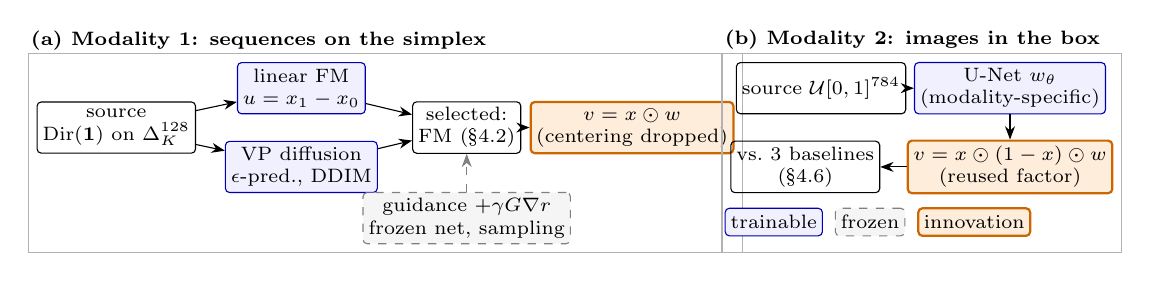
\begin{tikzpicture}[font=\scriptsize, >=Stealth,
  box/.style={draw, rounded corners=1.5pt, align=center, inner sep=2pt, minimum height=6.5mm},
  train/.style={box, draw=blue!70!black, fill=blue!6},
  frozen/.style={box, draw=gray, dashed, fill=gray!8},
  key/.style={box, draw=orange!80!black, fill=orange!14, line width=0.8pt}]
  % (a) Modality 1
  \node[box]    (src) at (0,0)      {source\\$\mathrm{Dir}(\mathbf 1)$ on $\Delta_K^{128}$};
  \node[train]  (fm)  at (2.35,0.5) {linear FM\\$u=x_1-x_0$};
  \node[train]  (df)  at (2.35,-0.5){VP diffusion\\$\epsilon$-pred., DDIM};
  \node[box]    (sel) at (4.45,0)   {selected:\\FM (\S4.2)};
  \node[key]    (inn) at (6.55,0)   {$v=x\odot w$\\(centering dropped)};
  \node[frozen] (gd)  at (4.45,-1.15){guidance $+\gamma G\nabla r$\\frozen net, sampling};
  \draw[->] (src) -- (fm); \draw[->] (src) -- (df);
  \draw[->] (fm) -- (sel); \draw[->] (df) -- (sel); \draw[->] (sel) -- (inn);
  \draw[->, dashed, gray] (gd) -- (sel);
  \node[draw=gray!60, fit=(src)(fm)(df)(sel)(inn)(gd), inner sep=3pt] (pa) {};
  \node[anchor=south west, font=\scriptsize\bfseries, inner sep=1pt] at (pa.north west) {(a) Modality 1: sequences on the simplex};
  % (b) Modality 2
  \node[box]    (s2) at (8.95,0.5)   {source $\mathcal U[0,1]^{784}$};
  \node[train]  (un) at (11.35,0.5)  {U-Net $w_\theta$\\(modality-specific)};
  \node[key]    (i2) at (11.35,-0.5) {$v=x\odot(1-x)\odot w$\\(reused factor)};
  \node[box]    (cp) at (8.75,-0.5)  {vs.\ 3 baselines\\(\S4.6)};
  \draw[->] (s2) -- (un); \draw[->] (un) -- (i2); \draw[->] (i2) -- (cp);
  \node[draw=gray!60, fit=(s2)(un)(i2)(cp)(gd.south -| cp.west), inner sep=3pt] (pb) {};
  \node[anchor=south west, font=\scriptsize\bfseries, inner sep=1pt] at (pb.north west) {(b) Modality 2: images in the box};
  % legend
  \node[train, minimum height=3.5mm]  (l1) at (8.35,-1.2) {trainable};
  \node[frozen, minimum height=3.5mm, right=1.5mm of l1] (l2) {frozen};
  \node[key, minimum height=3.5mm, right=1.5mm of l2] (l3) {innovation};
\end{tikzpicture}
}
\end{center}
\textbf{The pipeline.} Establish both baselines under one protocol $\rightarrow$ select a
family (4.2) $\rightarrow$ show controllability (4.3) $\rightarrow$ measure the pathology
$\rightarrow$ decompose the candidate fix and ablate it one piece at a time (4.4)
$\rightarrow$ position against three recent external methods (4.5) $\rightarrow$ transfer the
surviving mechanism to a second, unrelated bounded geometry (4.6).

\medskip
\srcs{Original figure (paper Fig.~1).}
\note{Audhav. Walk the arrow chain once, left to right; this is the map for Parts 2 and 3.}
\end{frame}

% ===================================================================== PART 2
% Speaker: Chang-Uk (2a-2c)

\begin{frame}{Choosing the base model}
\lab{2a}
\textbf{Decision rule, fixed before running:} lower marginal KL at NFE${=}10$.
\textbf{Confirmed on the real sequences} (dilated CNN, \RealSeeds{} seeds):
\begin{center}\tiny\resizebox{\linewidth}{!}{\begin{tabular}{lrrrrr}
\toprule
Dataset & FM, NFE 10 & Diff., NFE 10 & Diff.$-$FM, NFE 10 & Diff.$-$FM, NFE 100 & $x_0$ out (FM / Diff.) \\
\midrule
DNA ($K{=}4$) & 0.0061 $\pm$ 0.0043 & 0.7259 $\pm$ 0.4016 & $\mathbf{+0.720}$ [+0.447, +1.005] & +0.119 [+0.054, +0.194] & 0.979 / 0.993 \\
Protein ($K{=}20$) & 0.3120 $\pm$ 0.0632 & 2.2958 $\pm$ 0.4275 & $\mathbf{+1.984}$ [+1.724, +2.265] & +0.301 [+0.220, +0.391] & 1.000 / 1.000 \\
Codon ($K{=}64$) & 0.7483 $\pm$ 0.1314 & 1.7055 $\pm$ 0.6730 & $\mathbf{+0.957}$ [+0.570, +1.415] & +0.647 [+0.375, +0.991] & 1.000 / 1.000 \\
\bottomrule
\end{tabular}}\end{center}

\textbf{Selection.} Flow matching, better on \RealMinWins/\RealSeeds{} seeds at every NFE on
every dataset. The preregistered synthetic run agreed but used a small MLP and no real
data --- a disclosed deviation, and the reason for this confirmation.

\medskip
\textbf{The honest counterweight.} Diffusion was untuned (harness sized for flow matching), so
we claim the ordering, not the margin. On protein, 3-mer $r$ at NFE${=}10$ favours diffusion
(\RealProtKmerDiff{} vs \RealProtKmerFM), and on DNA and codon a unigram sampler already reaches
KL \UniKLDNA--\UniKLCodon, so this metric mostly tests composition.

\medskip
\textbf{And the finding that set up the rest of the talk:} the $x_0$-outside rate is the same
for both families --- \RealXDnaFM{} vs \RealXDnaDiff{} on DNA, \RealXCodonFM{} for both on
codon. \textbf{The pathology is not a property of one objective.}
\srcs{Tables regenerated from \texttt{results/fmdiff\_real\_*.jsonl} and
\texttt{results/fm\_vs\_diffusion.jsonl}; our own runs.}
\note{Chang-Uk. Do not skip the counterweight --- it is the fair-study point and it is graded.
If asked about the synthetic ``few-step'' result: it did not survive on real data; at
NFE=100 the gap is \RealCIHDna{} (DNA), \RealCIHProt{} (protein), \RealCIHCodon{} (codon).}
\end{frame}

\begin{frame}{Guidance works --- and what it costs}
\lab{2b}
\textbf{Setup.} The frozen \textbf{innovation model} ($x\odot w_\theta$) on real sequences; drift
$x\odot w_\theta+\gamma\nabla r$, then simplex projection (Euclidean rule), $\gamma$ constant; reward
$r=\sum_l\log\sum_{i\in S}x_{l,i}$ toward \textbf{GC content} (DNA) and \textbf{hydrophobic
fraction} (protein). Nothing retrained; \GRSeeds{} seeds, 4{,}000 samples.
\begin{center}\tiny\resizebox{0.62\linewidth}{!}{\begin{tabular}{lrrrrrr}
\toprule
& \multicolumn{3}{c}{DNA (GC)} & \multicolumn{3}{c}{Protein (hydrophobic)} \\
\cmidrule(lr){2-4}\cmidrule(lr){5-7}
$\gamma$ & Hit$\uparrow$ & $r_{\text{top}}\uparrow$ & Ham. & Hit$\uparrow$ & $r_{\text{top}}\uparrow$ & Ham. \\
\midrule
0 (unguided) & 0.09 & 0.59 & 0.75 & 0.03 & 0.60 & 0.94 \\
0.03 (low) & 0.30 & 0.92 & 0.74 & 0.55 & 0.74 & 0.94 \\
0.3 (default) & 1.00 & 0.65 & 0.53 & 1.00 & 0.53 & 0.84 \\
3 (high) & 1.00 & 0.55 & 0.44 & 1.00 & 0.50 & 0.72 \\
\midrule
\emph{Held-out real} & 0.09 & --- & 0.75 & 0.10 & --- & 0.94 \\
\bottomrule
\end{tabular}}\end{center}

\textbf{Controllability is established:} at $\gamma{=}0.3$ the hit rate (above the real 90th
percentile) rises by \GRHitCIDna{} (DNA) and \GRHitCIProt{} (protein), with no violations and no
extra runtime.

\medskip
\textbf{The cost is diversity and realism.} Hamming falls by \GRHamCIDna{} / \GRHamCIProt; strong
guidance overshoots real high-property sequences. Post hoc, the sweet spot is small $\gamma$:
similarity to the real top decile rises \GRKmerHiZeroDna{}$\rightarrow$\GRKmerHiMidDna{} on DNA at
$\gamma{=}\GRBestGammaDna$.
\srcs{Table from \texttt{results/guidance\_real\_*.jsonl}; our own runs.}
\note{Chang-Uk. Say plainly that the registered default (0.3) overshoots; the useful range is
0.03--0.1. The synthetic appendix check is where the exact ideal law and the gamma=0 violation
rate (the base field leaves the domain) live.}
\end{frame}

\begin{frame}{The innovation: which half of the fix works?}
\lab{2c}
\textbf{Motivation --- the measured pathology.} The learned field leaves the simplex on
$\BaseViolTwoDna$ of steps at $K{=}4$, $\BaseViolTwoProt$ at $K{=}20$, $\BaseViolTwoCodon$ at $K{=}64$ (the rate
counts any of $128K$ coordinates, so per coordinate it \emph{falls}). On a synthetic $K{=}\SweepK$ model the rate is flat
($\SweepRateLo$--$\SweepRateHi$) over a $\SweepRatio\times$ step-size sweep --- a property of the \emph{fit};
on real DNA it still rises from $\BaseViolDnaTen$ at NFE 10.

\medskip
\textbf{Specification.} The replicator parameterisation\,[1] is
$v = x \odot (w - \langle x, w \rangle)$ --- and it bundles \emph{two} distinct mechanisms:
\begin{itemize}
\item the factor $x_i$ makes each component vanish on the face $x_i = 0$ (the flow cannot exit)
\item the centering $\langle x, w\rangle$ gives $\sum_i v_i = 0$ (stay on the affine hull)
\end{itemize}
\textbf{Not separated in flow matching}; Wang \& Kanamori\,[2] use the same face-vanishing factor for
reflected score learning. We test the factor \emph{alone}:
\[
\textbf{mult-only } v = x \odot w, \qquad \textbf{center-only } v = w - \bar{w},
\]
against the base $v = w$ and the full form. Adds no parameters and no hyperparameters.
\srcs{[1] Boll et al.\ 2024, arXiv:2406.04527 --- the parameterisation is theirs, not ours \quad [2] Wang \& Kanamori 2026, arXiv:2608.03469}
\note{Chang-Uk. Be explicit that the parameterisation is prior art and the \emph{decomposition}
is ours. Expect a Q\&A question here.}
\end{frame}

% Speaker: Pedram (2d-2e)

\begin{frame}{Testing the innovation: one piece at a time}
\lab{2d}
\begin{center}\tiny\begin{tabular}{lrrrrrr}
\toprule
& \multicolumn{3}{c}{3-mer $r$} & \multicolumn{3}{c}{step violation} \\
\cmidrule(lr){2-4}\cmidrule(lr){5-7}
Arm & $K{=}4$ & $K{=}20$ & $K{=}64$ & $K{=}4$ & $K{=}20$ & $K{=}64$ \\
\midrule
base $w$ & 0.894 & 0.753 & 0.127 & 0.713 & 0.967 & 1.000 \\
mult $x \odot w$ & 0.899 & \textbf{0.865} & \textbf{0.196} & \textbf{0.0000} & \textbf{0.0000} & \textbf{0.0000} \\
center $w - \bar{w}$ & 0.910 & 0.777 & 0.120 & 0.721 & 0.967 & 1.000 \\
full replicator & 0.896 & \textbf{0.836} & \textbf{0.187} & 0.010 & 0.010 & 0.016 \\
\bottomrule
\end{tabular}\end{center}
\textbf{The multiplicative factor does the work.} Mult-only improves over base by
\MultCIProt{} at $K{=}20$ and \MultCICodon{} at $K{=}64$ on held-out data --- \MultProtPos/\MultProtN{}
and \MultCodonPos/\MultCodonN{} seeds; $t$-intervals agree. Violation is $\MultViolMax$ at
NFE $\ge 50$; $\MultViolTenLo$--$\MultViolTenHi\%$ at NFE 10, about one step in ten, consistent with the last.

\medskip
\textbf{Center-only is inert} --- non-significant at every $K$ (the base target already sums to
zero). The full replicator also helps, and \textbf{dropping its centering changes nothing}
(\DropCenterCICodon{} at $K{=}64$).

\medskip
\textbf{The clamping confound is not ruled out.} A gain from avoiding the clamp shrinks as NFE grows.
At $K{=}20$ ours does ($\MultMeanProtTen\rightarrow\MultMeanProtHundred$); at $K{=}64$ it is not
significant at NFE 10 and appears from NFE 50.
\srcs{Table regenerated from \texttt{results/endpoint\_*.jsonl}; \MOneSeeds{} seeds, our own runs. Bolding computed from the intervals.}
\note{Pedram. State the K=20 decay yourself before a panellist does: part of the gain may be
avoided clamping. The factor's gain is the robust one (8/8 seeds at K=20 and 64).}
\end{frame}

\begin{frame}{Position against recent work}
\lab{2e}
\begin{center}\tiny\resizebox{0.92\linewidth}{!}{\begin{tabular}{lrrrr}
\toprule
& \multicolumn{3}{c}{3-mer $r$ $\uparrow$ (NFE 100)} & Step viol. $\downarrow$ \\
\cmidrule(lr){2-4}
Method & DNA ($K{=}4$) & Protein ($K{=}20$) & Codon ($K{=}64$) & $K{=}4/20/64$ \\
\midrule
Dirichlet FM~\citep{stark2024dirichlet} & 0.901 $\pm$ 0.062 & 0.906 $\pm$ 0.020 & 0.447 $\pm$ 0.020 & 0.00/0.00/0.00 \\
Fisher-Flow~\citep{davis2024fisher} & 0.909 $\pm$ 0.049 & 0.886 $\pm$ 0.016 & 0.295 $\pm$ 0.013 & 0.00/0.00/0.00 \\
Gumbel-Softmax FM~\citep{tang2025gumbel} & 0.894 $\pm$ 0.052 & 0.705 $\pm$ 0.061 & 0.400 $\pm$ 0.070 & 0.00/0.00/0.00 \\
\midrule
Linear FM (internal base) & 0.894 $\pm$ 0.088 & 0.753 $\pm$ 0.058 & 0.127 $\pm$ 0.023 & 0.71/0.97/1.00 \\
\textbf{Ours}: $v = x \odot w$ & 0.899 $\pm$ 0.061 & 0.865 $\pm$ 0.027 & 0.196 $\pm$ 0.016 & 0.00/0.00/0.00 \\
\midrule
\emph{Reference: unigram sampler (no model)} & -0.046 $\pm$ 0.025 & 0.900 $\pm$ 0.002 & 0.218 $\pm$ 0.002 & --- \\
\bottomrule
\end{tabular}}\end{center}
\textbf{Fair study.} Each baseline keeps its own path, objective and decoding; backbone, budget and
seeds matched; our re-implementations, nothing quoted.

\medskip
\textbf{We are not state of the art.} At $K{=}4$ all are within noise. At $K{=}20,64$ Dirichlet
FM\,[1] leads us by \DirichletVsOursProt{} and \DirichletVsOursCodon, Fisher-Flow\,[2] by
\FisherVsOursProt{} and \FisherVsOursCodon; we beat Gumbel-Softmax FM\,[3] only at $K{=}20$. A \textbf{unigram sampler} scores
$\UniProtein$ / $\UniCodon$: protein is near its composition floor; on codon ours is below it.

\medskip
\textbf{Feasibility does not separate them:} all three are feasible in their own samplers.
\srcs{[1] St\"ark et al.\ 2024, ICML \quad [2] Davis et al.\ 2024, NeurIPS \quad [3] Tang et al.\ 2025}
\note{Pedram. Say "we are not state of the art" in plain words. If asked about corrections:
our first Fisher-Flow sampler integrated a sphere velocity in simplex coordinates, and our first
Dirichlet and Gumbel arms trained on wrong velocity targets (Gumbel's 18x too small). All three
were corrected by preregistered reruns; the old rows are disclosed in the appendix. The old
"we beat Gumbel and Dirichlet" and "best method violates every step" were artefacts of those bugs.}
\end{frame}

% ===================================================================== PART 3
% Speakers: 3a Audhav, 3b Pedram, 3c Chang-Uk, 3d Pedram, 3e Roshan (see slides/README.md)

\begin{frame}{The transferred method}
\lab{3a}
\textbf{What stays exactly the same.} The mechanism is a parameterisation of the
\emph{velocity}, not an architecture --- so it transfers verbatim in form. The invariant idea is
\emph{a factor that vanishes where the domain ends}:
\[
\text{simplex: } v = x \odot w \qquad \longrightarrow \qquad
\text{box: } v = x \odot (1-x) \odot w ,
\]
vanishing at \emph{both} faces of every interval. Still no added parameters, no added
hyperparameters, same loss, same preregistered protocol.

\medskip
\textbf{What changes, and why it is not the mechanism.} The box has no sum-to-one constraint, so
there is no centering term to drop --- \textbf{the box arm \emph{is} the mult-only form}, which
is precisely why Modality 2 tests the half of the innovation that survived Part 2.

\medskip
\textbf{Training.} U-Net backbone (two down stages, mid block, symmetric up with skips,
GroupNorm, SiLU, sinusoidal time embedding per block), Adam lr $2{\times}10^{-4}$, batch 128,
\MTwoSteps{} steps, \MTwoSeeds{} seeds, \MTwoEval{} evaluation samples (\MTwoParams{} parameters).

\medskip
\textbf{Sampling.} Euler at NFE $\in \{10,50,100\}$; violations counted on the \emph{unclamped}
update, exactly as in Modality 1.
\srcs{Architecture and protocol are ours; no external code or checkpoint used in this arm.}
\note{Audhav. Stress the "is the mult-only form" line --- it is what makes this one mechanism on
two geometries rather than two mechanisms.}
\end{frame}

\begin{frame}{Transfer results}
\lab{3b}
\begin{center}\tiny\begin{tabular}{lrrrrr}
\toprule
Method & FD $\downarrow$ & Coverage $\uparrow$ & Density $\uparrow$ & FD@10 $\downarrow$ & Step viol. $\downarrow$ \\
\midrule
Reflection sampler~\citep{lou2023reflected} & 192.0 $\pm$ 143.5 & 0.624 & 0.478 & 540.3 & 0.1401 \\
Mirror-map FM~\citep{liu2023mirror} & 52.5 $\pm$ 23.9 & 0.685 & 0.480 & 98.9 & 0.0000 \\
Dyn.\ thresholding on $x_t$~\citep{saharia2022imagen} & 195.5 $\pm$ 150.3 & 0.623 & 0.480 & 540.8 & 0.1604 \\
\midrule
Flow matching (internal base) & 193.9 $\pm$ 145.6 & 0.623 & 0.478 & 545.3 & 0.1602 \\
\textbf{Ours}: $v = x(1-x)\odot w$ & 151.0 $\pm$ 47.4 & 0.410 & 0.302 & 269.6 & 0.0000 \\
\bottomrule
\end{tabular}\end{center}
\textbf{Fair study.} Matched backbone, optimiser, schedule, batch, steps, seeds and evaluation
count across all five arms. The three external arms are \textbf{our flow-matching
re-implementations}\,[1,2,3]: reflection and thresholding are sampler rules on the base network,
mirror trains in logit space --- none is the published diffusion model. Quality is Fr\'echet distance in the feature space of a
classifier we train ourselves, and \textbf{we report its test accuracy} ($\MTwoAcc\%$; one classifier, shared by every arm) because our critique of this field's metrics applies to ours too. Diversity is coverage\,[4].

\medskip
\textbf{Fair discussion.} See the following slide --- the result is mixed, and the parts that go
against us are on it.
\srcs{[1] Lou \& Ermon 2023, ICML \quad [2] Liu et al.\ 2023, NeurIPS \quad [3] Saharia et al.\ 2022 \quad [4] Naeem et al.\ 2020, ICML}
\note{Pedram. Read the table, then hand straight to 3c for the verdict.}
\end{frame}

\begin{frame}{Does the innovation transfer?}
\lab{3c}
\textbf{Direction and magnitude, compared across modalities.}
\begin{itemize}
\item \textbf{Feasibility transfers.} Step violation is $\MTwoViolOurs$ on the box at NFE 100, as on
the simplex. Same mechanism, unrelated geometry --- this part is unambiguous.
\item \textbf{Quality does \emph{not} transfer.} Against the internal base, \MTwoClaim{}
over \MTwoSeeds{} seeds --- \textbf{contains zero}, so on our preregistered rule the transfer claim
is \textbf{not supported}. Mirror-map FM beats us significantly (\MTwoVsMirror); we lose
coverage and density on $\MTwoCovLosses$ and $\MTwoDensLosses$ of $\MTwoSeeds$ seeds; reflection and thresholding act as plain clamping.
\item \textbf{The mean rests on one seed.} Ours wins FD on $\MTwoWins$ of $\MTwoSeeds$ seeds; drop seed
$0$ and $\MTwoClaimMean$ becomes $\MTwoDropSeedZeroMean$. Its spread is lower (s.d.\ $\MTwoSdOurs$ vs
$\MTwoSdBase$; exploratory, untested), and FD at NFE 10 is lower on $\MTwoFDTenWins$ seeds --- a gain
that vanishes as steps shrink.
\item \textbf{We refuted our own explanation of the cost.} We had said image data are
\emph{interior}, so the factor is free there. Measuring it: only $\MTwoInteriorPct\%$ of MNIST pixels are interior, and $x(1-x)$ is
throttled below a tenth of its maximum on $\MTwoThrottledPct\%$ of them. \textbf{Both} modalities are
boundary-concentrated; the cost is paid wherever data concentrate at the boundary.
\end{itemize}

\textbf{Verdict.} \emph{Feasibility} transfers, for the same reason, in both geometries.
\emph{Quality} does not --- the transfer claim fails its own preregistered test.
\srcs{Mirror: Liu et al.\ 2023 \quad Reflection: Lou \& Ermon 2023 \quad Thresholding: Saharia et al.\ 2022}
\note{Chang-Uk. Give the verdict in one sentence and resist overclaiming. This is graded on
matching the claim to the evidence.}
\end{frame}

\begin{frame}{Limitations and failure modes}
\lab{3d}
\begin{enumerate}
\item \textbf{The factor still overshoots at few steps.} At NFE 10, Euler exits on
$\MultViolTenLo$--$\MultViolTenHi\%$ of steps, and at $K{=}64$ it gives no gain there.
\item \textbf{Constraint satisfaction does not buy quality.} Every strong method is feasible ---
Dirichlet and Gumbel by vanishing mixtures, Fisher-Flow and mirror by coordinates --- and they still
differ widely; on protein no arm beats composition by much, and on codon ours is below it.
\item \textbf{On images we lose both fidelity and diversity}: density and coverage are lower on
$\MTwoDensLosses$ and $\MTwoCovLosses$ of $\MTwoSeeds$ seeds, and samples are visibly blotchier.
\item \textbf{High seed variance on Modality 2.} Three of five arms swing by almost an order of
magnitude between seeds, which is why the seed count was raised $3 \rightarrow 8$ by dated
amendment before reading the remaining seeds.
\item \textbf{Six interventions were falsified}, and we report them: the Modality~2 quality transfer, a soft tangency penalty,
a convex-combination integrator (a no-op), a $(1-t)^2$ loss reweighting that was
\emph{harmful} (\ReweightCIProt{} vs.\ base; the $t$-interval includes zero), the endpoint
parameterisation and the centering term.
\item \textbf{Scale.} All models are small ($\approx$0.6M parameters); a larger backbone was tried
only on superseded data.
\end{enumerate}
\srcs{All figures from our own runs and preregistration log.}
\note{Pedram. About 8 seconds per item; do not read them out in full.}
\end{frame}

\begin{frame}{Conclusions and next steps}
\lab{3e}
\textbf{Back to the motivation.} The tangency premise confined-flow theory assumes\,[1] does not
carry over to \emph{learned} fields: violation is the norm ($\BaseViolTwoDna$--$\BaseViolTwoCodon$ of
steps) in both generative families --- but \textbf{every strong method is feasible}, by mixtures or
by coordinates.

\medskip
\textbf{Mechanism.} Of the two pieces bundled in the replicator form, only the multiplicative factor
does anything; the centering term is inert, so \textbf{it can be dropped}.
The likeliest reading is an inductive bias, not the constraint; part of the $K{=}20$ gain may be
avoided clamping.

\medskip
\textbf{The narrowest claim we can defend.} A vanishing factor removes violation (at NFE $\ge50$) at
no parameter cost and improves a linear flow at $K\ge20$; its centering is unnecessary; it does not
close the gap to recent methods, and on images it transfers feasibility but not quality.

\medskip
\textbf{Next experiment.} The factor at a larger backbone on the held-out split --- does its
gain survive scale?
\srcs{[1] Cont 2026, arXiv:2607.28344 (Assumption F4)}
\note{Roshan. Close on the next experiment, not on the win. Leaves the panel a question we
have already thought about.}
\end{frame}

% ===================================================================== bibliography

\begin{frame}{Bibliography (1/3)}
\lab{Refs}
\footnotesize
\begin{itemize}\itemsep1pt
\item Albergo, M.S., Boffi, N.M., Vanden-Eijnden, E. Stochastic interpolants: a unifying
framework for flows and diffusions. \emph{JMLR} 26(209), 2025.
\item Boll, B., Gonzalez-Alvarado, D., Petra, S., Schn\"orr, C. Generative assignment flows for
representing and learning joint distributions of discrete data. arXiv:2406.04527, 2024.
\item Cont, R. Reflected diffusions, no-flux continuity equations and confined Lagrangian flows
in bounded domains. arXiv:2607.28344, 2026.
\item Davis, O., Kessler, S., Petrache, M., Ceylan, \.I.\.I., Bronstein, M., Bose, A.J. Fisher
flow matching for generative modeling over discrete data. \emph{NeurIPS} 37, 2024.
\item Eijkelboom, F., Bartosh, G., Naesseth, C.A., Welling, M., van de Meent, J.-W. Variational
flow matching for graph generation. \emph{NeurIPS}, 2024.
\item Ensembl. Ensembl 2023. \emph{Nucleic Acids Research} 51(D1), 2023.
\item Fishman, N., Klarner, L., De Bortoli, V., Mathieu, E., Hutchinson, M. Diffusion models for
constrained domains. \emph{TMLR}, 2023.
\item Ho, J., Salimans, T. Classifier-free diffusion guidance. arXiv:2207.12598, 2022.
\item Karras, T., Aittala, M., Aila, T., Laine, S. Elucidating the design space of
diffusion-based generative models. \emph{NeurIPS} 35, 2022.
\end{itemize}
\end{frame}

\begin{frame}{Bibliography (2/3)}
\lab{Refs}
\footnotesize
\begin{itemize}\itemsep1pt
\item LeCun, Y., Bottou, L., Bengio, Y., Haffner, P. Gradient-based learning applied to document
recognition. \emph{Proc.\ IEEE} 86(11), 1998.
\item Lipman, Y., Chen, R.T.Q., Ben-Hamu, H., Nickel, M., Le, M. Flow matching for generative
modeling. arXiv:2210.02747, 2022.
\item Liu, G.-H., Chen, T., Theodorou, E.A., Tao, M. Mirror diffusion models for constrained and
watermarked generation. \emph{NeurIPS}, 2023.
\item Lou, A., Ermon, S. Reflected diffusion models. \emph{ICML}, 2023.
\item Naeem, M.F., Oh, S.J., Uh, Y., Choi, Y., Yoo, J. Reliable fidelity and diversity metrics
for generative models. \emph{ICML}, 2020.
\item Nichol, A.Q., Dhariwal, P. Improved denoising diffusion probabilistic models. \emph{ICML},
2021.
\item Saharia, C., et al. Photorealistic text-to-image diffusion models with deep language
understanding (Imagen). \emph{NeurIPS} 35, 2022.
\item Song, J., Meng, C., Ermon, S. Denoising diffusion implicit models. \emph{ICLR}, 2021.
\item St\"ark, H., Jing, B., Wang, C., Corso, G., Berger, B., Barzilay, R., Jaakkola, T.
Dirichlet flow matching with applications to DNA sequence design. \emph{ICML}, 2024.
\end{itemize}
\end{frame}

\begin{frame}{Bibliography (3/3)}
\lab{Refs}
\footnotesize
\begin{itemize}\itemsep1pt
\item Tang, S., Zhang, Y., Tong, A., Chatterjee, P. Gumbel-softmax flow matching with
straight-through guidance. arXiv:2503.17361, 2025.
\item UniProt Consortium. UniProt: the universal protein knowledgebase in 2023. \emph{Nucleic
Acids Research} 51(D1), 2023.
\item Wang, Z., Kanamori, T. Should the boundary term be learned in reflected diffusion? Conormal
trace and reflection masking. arXiv:2608.03469, 2026.
\item Wang, C., Uehara, M., He, Y., et al. Fine-tuning discrete diffusion models via reward
optimization (DRAKES). \emph{ICLR}, 2025.
\item Wang, W., Carreira-Perpi\~n\'an, M.\'A. Projection onto the probability simplex.
arXiv:1309.1541, 2013.
\item Xie, T., Zhu, Y., Yu, L., Yang, T., Cheng, Z., Zhang, S., Zhang, X., Zhang, C. Reflected flow
matching. \emph{ICML}, 2024.
\item Zern, A., Schn\"orr, C. On the correspondence between replicator dynamics and assignment
flows. \emph{SSVM}, 2021.
\end{itemize}
\end{frame}

\end{document}
